\chapter*{Resumen}
En el presente trabajo se integra un conjunto de software de código libre con el objetivo de proponer e implementar un ambiente de simulación para software in the loop, que permita la validación de un sistema de misión de vuelo de un quadrotor autónomo virtual; el sistema en cuestión se encuentra integrado por dos grandes partes, por un lado, se tiene un algoritmo de visión por artificial para la detección de un tipo de compuerta utilizado en las competencias de drones autónomos para delimitar circuitos de vuelo, y por otro lado, se implementa un algoritmo de seguimiento de trayectoria basado en waypoints, en donde un script se comunica con un firmware de piloto automático, de tal forma que se envían comandos de vuelo específicos para que el dron sea capaz pasar a través de una serie de compuertas y completar la trayectoria que define el circuito vuelo.

Así mismo, dentro de la simulación se pueden destacar dos componentes de gran relevancia, el circuito de vuelo y el dron virtual. La figura \ref{fig:method} presenta un esquema de alto nivel del sistema que se implementa en la simulación. 

El circuito de vuelo se describe con 4 compuertas posicionadas en un arreglo rectangular simple y el dron virtual cuenta con una cámara simulada, a partir de la cual se extrae la trama de video para el algoritmo de segmentación, y un plugin para el piloto automático que le permite recibir comando de vuelo para volar a través del circuito.

\begin{figure}[ht]
    \centering
    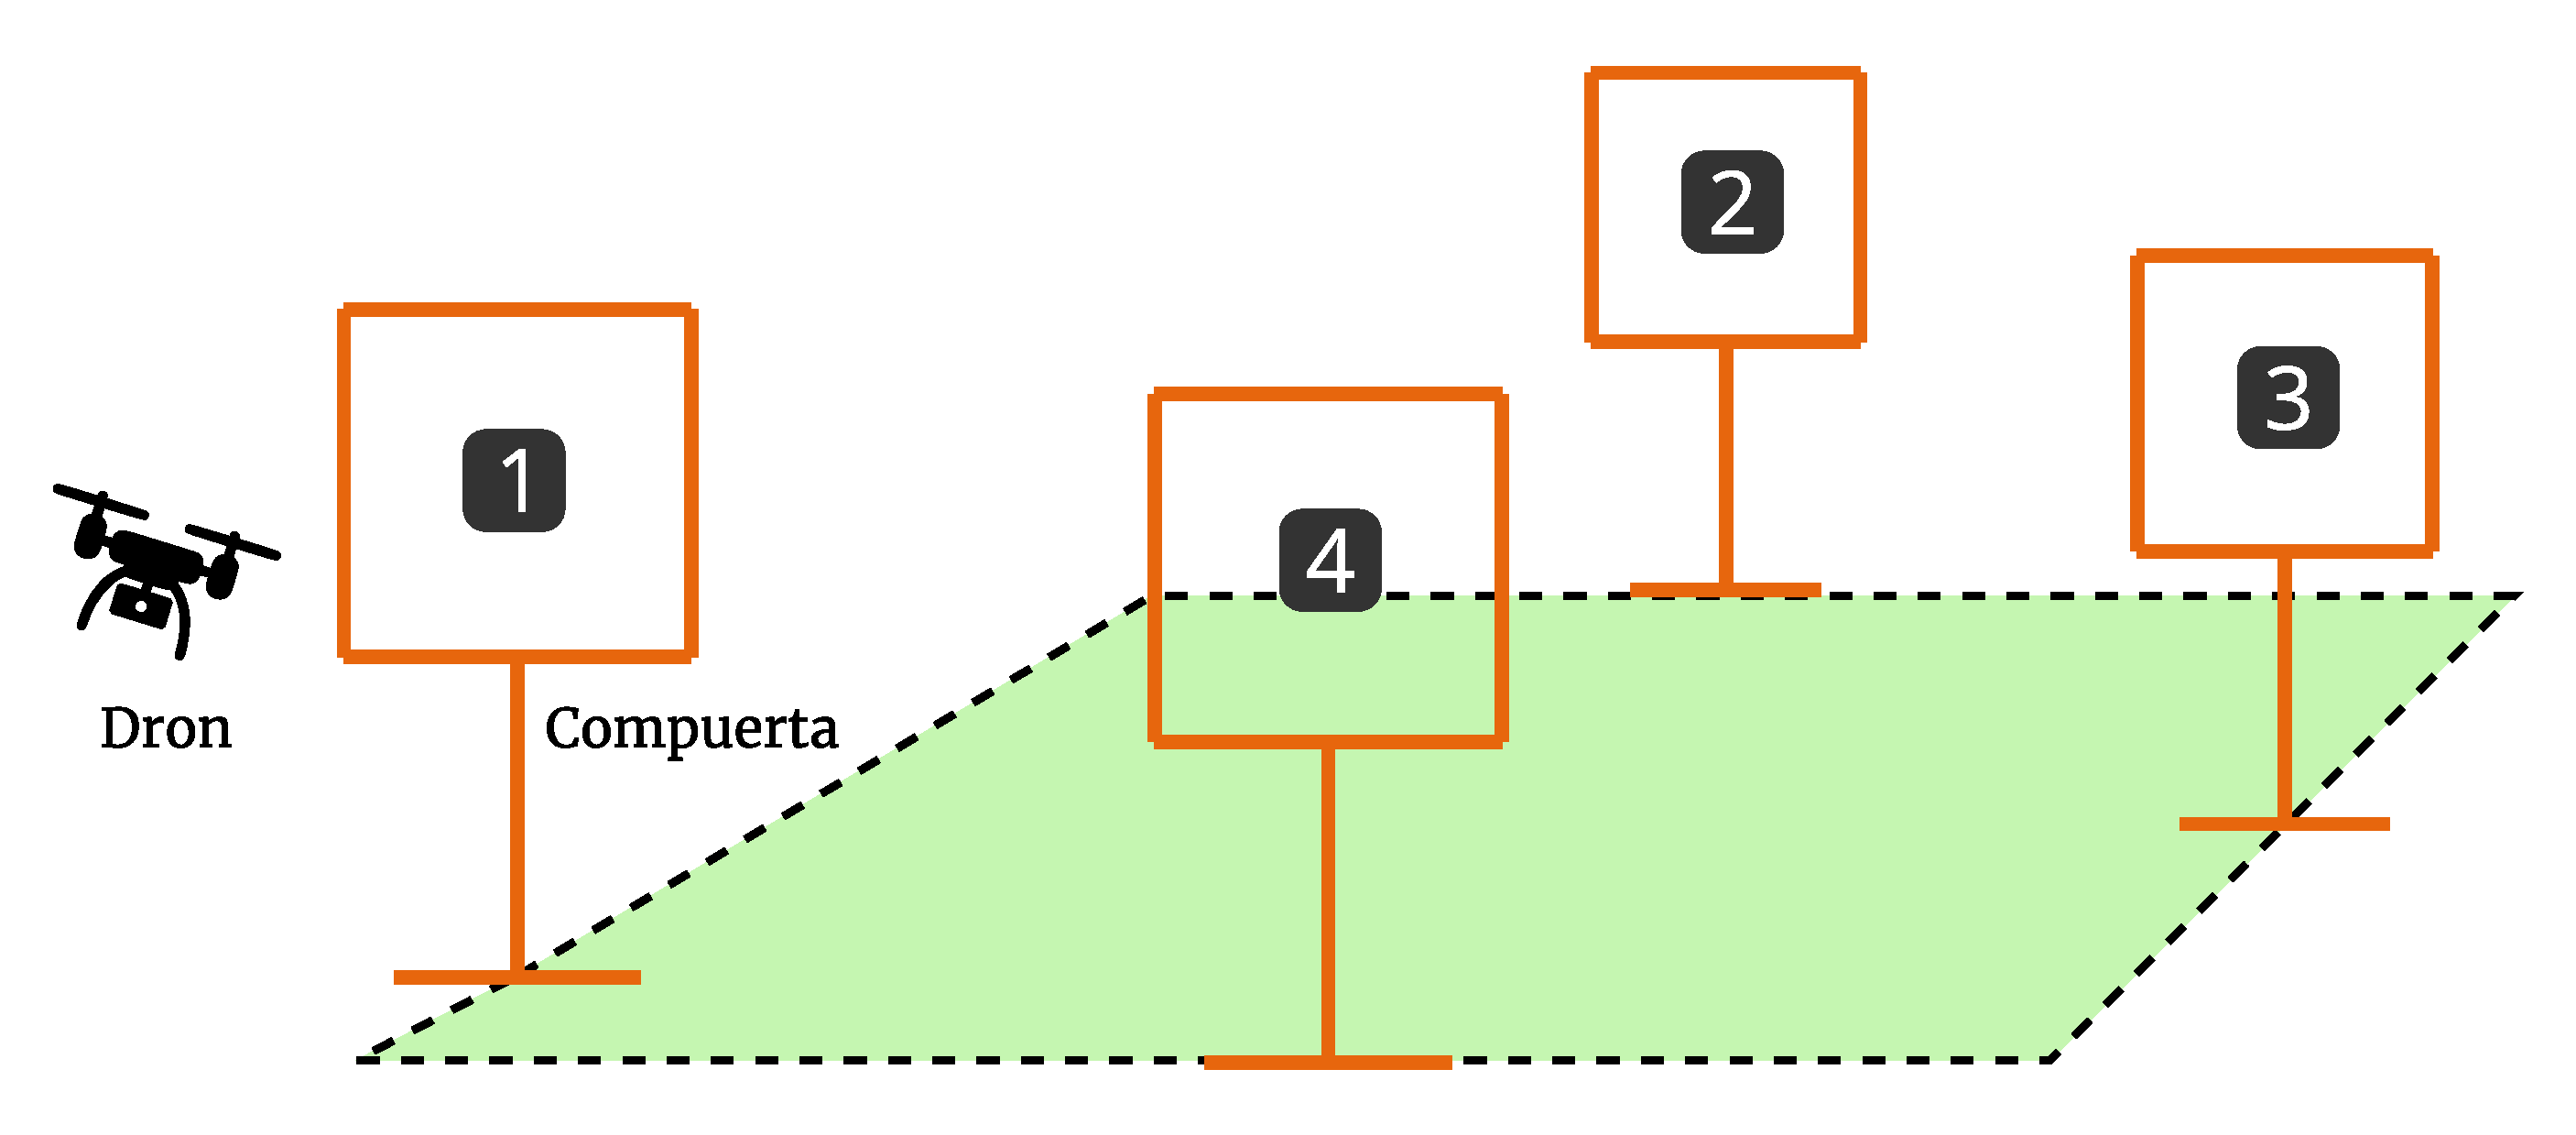
\includegraphics[width=0.8\textwidth]{Method.pdf}
    \caption{Diagrama general de los componentes de la simulación}
    \label{fig:method}
\end{figure}

Adicionalmente, y como se mencionó anteriormente, el sistema de misión de vuelo se conforma por un conjunto de software y librerías de última generación, las cuales se describen a continuación.

\textbf{OpenCV}: una librería robusta para aplicaciones de visión artificial, con la cual se llevó a cabo la implementación del algoritmo de detección de compuertas.

\textbf{PymavLink}: una librería que cuenta con una API basada en el protocolo de comunicación MAVLink. Esta permitió la comunicación con el firmware de piloto automático, ArduPilot.

\textbf{Gazebo}: un ambiente de simulación con gráficas en 3D, pensado para aplicaciones del área de robótica, en él se elaboró el circuito de vuelo. 

\textbf{ArduPilot}: un firmware para pilotos automáticos que ofrece herramientas para realizar simulación de software in the loop.

\textbf{ROS 2}: la nueva versión del framework de desarrollo de aplicaciones de robótica; parte esencial para la integración del sistema de misión de vuelo.

\textbf{GNU/Linux}:  el sistema operativo en donde se desarrolló el proyecto en su conjunto.


Por último, se documenta con gran detalle el proceso de integración de todas las herramientas de software utilizadas, así como el comportamiento final del sistema propuesto.










